\chapter{Marco Teórico}
\label{chap:marcoteorico}
%\endinput
% Estado del arte general de la temática de estudio. 
\section{Introducci\'on}

Para el an\'alisis de posibles colisiones es necesario evaluar de forma anticipada las trayectorias de todos los objetos que orbitan la Tierra y detectar los acercamientos de riesgo. Si la predicci\'on de las posiciones fuera exacta, este estudio s\'olo implicar\'ia un esfuerzo computacional a resolver. No obstante, el movimiento orbital de los objetos no es ideal y las posiciones medidas o estimadas siempre acarrean una indeterminaci\'on, y m\'as a\'un cuando se trata de desechos.\\

Las primeras t\'ecnicas de detecci\'on de encuentros, realizaban propagaciones de las posiciones una semana hacia el futuro, defin\'ian un volumen seguro rodeando al sat\'elite de inter\'es, y si alg\'un objeto externo se introduc\'ia dentro del volumen de riesgo, es decir, se acercaba a una distancia m\'inima por debajo del umbral determinado, se consideraba una situaci\'on de acercamiento que deb\'ia ser estudiada. Estas metodolog\'ias no ten\'ian en cuenta los errores en la determinaci\'on de la posici\'on de los objetos, y por lo general derivaban en falsas alarmas, con las que se corr\'ia el riesgo de realizar maniobras innecesarias.\\
En la actualidad, adem\'as de la m\'inima distancia de acercamiento o {\it{miss distance}}, se calcula la {\bf{probabilidad de colisi\'on}}: PoC.  Esta \'ultima ofrece un panorama m\'as completo de la situaci\'on ya que incorpora los errores en las posiciones a trav\'es de las matrices de covarianza.\\

Como ya mencionamos (Sec. \ref{subsec:estudiocolison}), en este trabajo nos enfocamos en analizar las situaci\'ones de encuentro ya identificadas y que involucran a misiones operativas y desechos espaciales.\\

La posici\'on de la misi\'on operativa y los errores asociados a la misma, la provee el departamento de din\'amica orbital (Sec. \ref{sec:posMision}).
La posici\'on de los desechos, s\'olo es posible conocerla, utilizamos los datos p\'ublicos que ofrece el comando de defensa norteamericano, \ac{NORAD} a trav\'es de su p\'agina Space-Track {\footnote{http://www.space-track.org}}. Las posiciones son publicadas en formato \ac{TLE} (Sec. \ref{sec:tleformat}), sin errores asociados, y son propagadas hasta el momento del encuentro con el modelo SGP4 (Sec. \ref{sec:sgp4model}), que tampoco ofrece informaci\'on sobre los errores de propagaci\'on.\\

En este cap\'itulo, en primer lugar presentamos la forma en que se comunican los acercamientos de riesgo (Sec. \ref{sec:anuncio}), por ejemplo mediante \ac{CDM}. Luego describimos las distintas determinaciones en las posiciones y los formatos en que se presentan y el modelo SGP4 para la propagaci\'on de los TLE.\\
Detallamos el m\'etodo de Osweiler \citep{Osweiler} que utilizamos para la contrucci\'on de las matrices de covarianzas correspondientes a los desechos y la generaci\'on e implementaci\'on de una tabla con valores estad\'isticos inferidos de an\'alisis de datos de misi\'on, para la propagaci\'on de la matriz de covarianza al momento del m\'aximo acercamiento.\\
Finalmente detallamos el algoritmo para el c\'alculo de la PoC.\\


\section{Comunicaciones de riesgos de colisi\'on}{\label{sec:anuncio}}

El CDM tuvo su precedente en el CSM {\it{Conjunction Summary Message}} (\textcolor{red}{citar bibliograf\'ia que lo describa y si sobra tiempo ampliar}).  es un mensaje enviado por JSpOC a los operadores o due\~nos de misi\'on cuando alguno de sus sat\'elites fue identificado en un acercamiento de riesgo con otro objeto del ambiente espacial.\\
El mismo fue acordado y promovido por el .... IADC y adoptado por el COPUOS en el a\~no, bajo los est\'andares que se describen en el blue book del CCSDS. \\
Los CDM se env\'ian a los operadores a cargo y/o se disponibilizan en la p\'agina de space-track para usuarios con permisos especiales 72 hs antes del encuentro. Para la generaci\'on de los mismos se consideran criterios de emergencia, seg\'un ocurra que el acercamiento entre los objetos es:\\

LEO:\\
overall miss distance < 1km\\
radial miss distance < 200m\\
GEO/MEO:\\
Overall miss distance < 10 km.\\

Son mensajes exclusivamente informativos, que no imprimen recomendaciones ni sugerencias de acci\'on.
Y es importante destacar que muchas veces para las estimaciones, los centros de c\'omputo no cuentan con maniobras planificadas en sus predicciones.\\ 

El mismo se distribuye en distintos formatos ...ampliar ...CCSDS standard para el CDM. \\
\textcolor{red}{Incorporar formato}

Con la recepci\'on de un CDM, uno ya puede entre otras cosas:\\
* identificar la misi\'on operativa involucrada.\\
* identificar el desecho involucrado.\\
* conocer el momento del m\'aximo acercamiento TCA.\\
* Conocer r, v en TCA?. en CRF, RTN??\\
* Las matrices de covarianzas de los errores.\\
* La PoC.\\

\section{La posici\'on de los objetos involucrados}{\label{sec:posMision}}

En nuestro planteo de riesgos por colisi\'on entre misiones operativas y desechos espaciales, existir\'an dos abordajes distintos del problema de la determinaci\'on de las posiciones, ya que cada uno de los objetos involucrados ofrece metodolog\'ias y modelos diferentes.

\subsection*{La posici\'on de la misi\'on operativa}
Con la misi\'on operativa tenemos contacto y comandado. En gral tiene un GPS o alg\'un otro instrumento de determinaci\'on de la posici\'on, con un cierto error asociado, que es conocido.({\bf{cu\'al?}})\\
A su vez CONAE tiene su modelo orbital de propagaci\'on y generaci\'on de predicci\'on (PREPHEM), y su propio modelo de ajuste (ORBEPHEM).\\

\subsection*{La posici\'on del desecho espacial}
El desecho espacial no tiene capacidades operativas, de manera que la \'unica manera de determinar su posici\'on es con redes de rastreo desde Tierra.\\
Caracter\'istica de las redes de rastreo. error asociado, que es conocido.({\bf{cu\'al?}})\\
S\'olo usa, rusia y la uni\'on europea cuentan con redes de rastreo. En particular Norad es la que disponibiliza en forma p\'ublica los datos en formato TLE.\\
Dado este contexto, las distintas agencias, que no cuentan con gran n\'umero de misiones operativas, suelen contratar/acordar este servicio. Y a\'un, con herramientas propias desarrolladas, lleva tiempo la validaci\'on de las mismas hasta lograr cierta autonom\'ia. No obstante, la tendencia es hacia un primer paso, que permita una caracterizaci\'on m\'as precisa de la situaci\'on de encuentro, sumando a la informaci\'on p\'ublica, m\'etodos de ajuste, datos propios de la misi\'on en riesgo y estimadores del riesgo como por ejemplo la \ac{PoC}.\\
Es en esa direcci\'on que planteamos este trabajo, a fin de ofrecer un prototipo que pueda ser implementado en paralelo a lo que ya se utiliza en CONAE, para ser probado y mejorado con la experiencia que sumen los encuentros que involucren a las misiones nacionales.\\
Describir:\\

\section{Los TLE}{\label{sec:tleformat}}

.....TLE FORMAT.

\subsection{SGP4}{\label{sec:sgp4model}}

\section{Estimaci\'on de Errores en la posici\'on}
Metodo de OSW.
\subsection{M\'etodo de Osweiler}
Es un m\'etodo que propone una manera de estimar los errores que se comenten en la utilizaci\'on de TLEs para la determinaci\'on de la posici\'on y la velocidad.
 El mismo consiste en utilizar un set de TLEs de un intervalo de dos semanas, y considerar el TLE m\'as pr\'oximo al tiempo de m\'aximo acercamiento (TLE  {\it{Primario}}) como el valor {\it{real}} o {\it{verdadero}}.\\
 A partir de esa premisa, propaga los TLEs anteriores hasta la \'epoca del TLE Primario y con las diferencias que resultan de la comparaci\'on, realiza los c\'alculos estad\'idticos de los valores medios y las varianzas, para construir la matriz Varianza Covarianza correpondiente al TLE Primario.\\
 Para hacer los estudios de validaci\'on de nuestra implementaci\'on del m\'etodo, de los 6 sat\'elites estudiados por Osweiler, dentro de 8 ventanas temporales distintas, nosotros hemos aplicado el m\'etodo a dos de ellos con caracter\'isticas similares a las misiones de CONAE y en particular a la misi\'on SAC-D, que hemos incorporamos como escenario propio de valiaci\'on ya que contamos con datos orbitales reales de mayor precisi\'on que los TLEs.

\subsection{Tratamiento sobre Datos de Misi\'on}
En esta etapa repetimos el m\'etodo que propone Osweiler considerando los datos de misi\'on generados por el CODS
como posici\'on verdadera.\\
La aplicaci\'on del m\'etodo implica:
\begin{itemize}
 \item Identificar el \'ultimo TLE del set: {\it{TLE primario.}}
 \item Extraer la \'epoca del TLE primario.
 \item Localizar el archivo CODS que contenga las efem\'erides que encierren la \'epoca del TLE primario.
 \item Interpolar las efem\'erides de CODS para generar una efem\'eride interpolada a la \'epoca del TLE primario.
 \item Propagar cada uno de los TLEs del set, hasta la \'epoca del TLE primario.
 \item Comparar los resultados de las propagaciones con los valores de la efem\'erides interpolada.
\end{itemize}

\begin{figure}[!h]
 \centering
 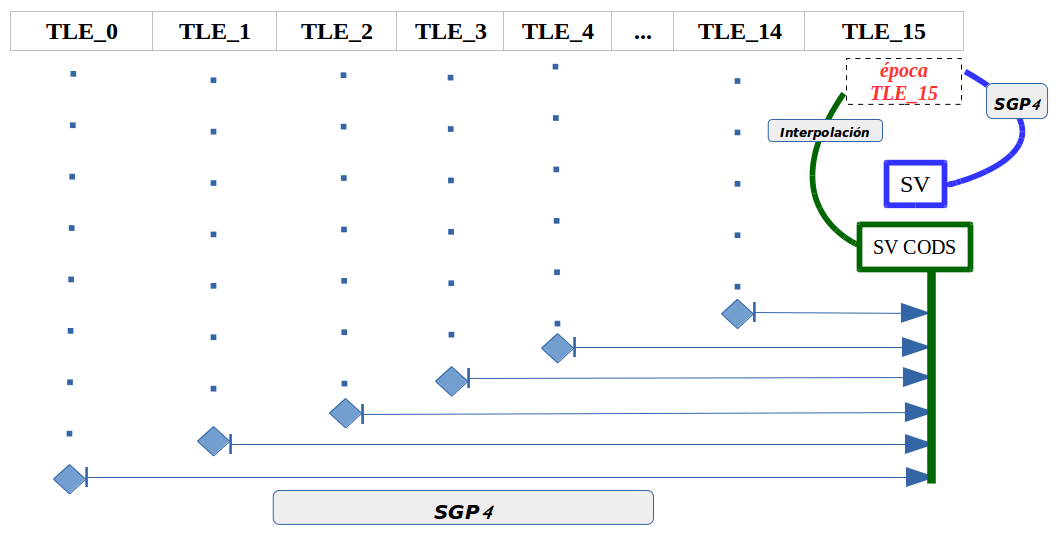
\includegraphics[width=0.7\textwidth]{imagenes/Osweiler_sobre_Cods.png}
 \caption{M\'etodo de Osweiler sobre datos CODS}
\end{figure}

\section{La Probabilidad de Colisi\'on}

Como ya hemos mencionado, el an\'alisis de una situaci\'on de riesgo puede realizarse tomando como par\'ametro:\\
\begin{itemize}
 \item La m\'inima distancia.
 \item La probabilidad de Colisi\'on (PoC).
 \item La m\'axima PoC.
\end{itemize}

Estos par\'ametros se calculan a partir de:
\begin{itemize}
 \item \'Orbitas Predichas.
 \item Covarianzas.
\end{itemize}

Luego se juzgan m\'argenes para las acciones a seguir seg\'un criterios propios del centro de control, que tiene en cuenta distintas consideraciones propias de la misi\'on.\\ 



{\bf{citar a Klinkrad}}
\\
Distintos autores han desarrollado varios m\'etodos para el c\'alculo de la PoC (Patera, Klinkrad, Akella \& Alfriend...etc..mencionar y detallar un poco), y todos ellos comparten las siguientes consideraciones:\\
\begin{itemize}
 \item El error en la posici\'on puede representarse por una funci\'on de distribuci\'on Gaussiana 3D, cuya funci\'on de densidad de probabilidad se detalla en la eq...{\bf{bla}} 
 \item Tanto el objeto primario, como el desecho se mueven en movimiento rectil\'ineo con velocidad constante durante el encuentro.
 \item Los errores en las velocidades se desprecian.
 \item Los errores en las posiciones del objeto primario y del desecho no est\'an correlacionados.
 \item Los errores en las posiciones son constantes durante el encuentro, al igual que la matrices de covarianzas correspondientes al TCA.
\end{itemize}

\subsection*{M\'etodo de Akella}
En este trabajo para el c\'alculo de la PoC se utilizar\'a el m\'etodo de Alfriend \& Akella[4] ya que es conceptualmente simple y aunque tiene un alto costo computacional, es realizable por las m\'aquinas actuales en tiempos menores a un segundo.\\

El mismo requiere como entradas:
\begin{itemize}
 \item Conocer el instante de m\'aximo acercamiento: TCA (Time of Closest Approach).
 \item La posici\'on relativa del desecho respecto al objeto primario en el TCA.
 \item La velocidad relativa del desecho respecto al objeto primario en el TCA.
 \item Las matrices de error de ambos objetos.
\end{itemize}

En los momentos pr\'oximos al encuentro, la posici\'on relativa de riesgo $\Delta r$ puede expresarse en funci\'on de un intervalo de tiempo respecto del TCA, es decir, $\Delta t_{tca}=t-t_{tca}$.

\begin{equation}
 \Delta r(t)=\Delta r_{tca}+\Delta v_{tca}(t-t_{tca})
\end{equation}

Las matrices de covarianza de los errores que son calculadas para un momento dado t previo al TCA, deben ser propagadas. ({\bf{ver metodolog\'ia}})
Dado que consideramos que los errores en las posiciones de ambos objetos no est\'an correlacionadas, ambas contribuciones pueden combinarse en una \'unica matriz, a partir de la suma de ambas.

\begin{equation}
 C=C_{p}+C_{d}
\end{equation}

De $C$ s\'olo consideraremos la submatriz superior de la izquierda de dimensiones (3x3), que corresponde a los errores en las posiciones, con un $1 \sigma$.\\
Dado que adem\'as asumimos que los errores en la posici\'on son de distribuci\'on normal en 3D, la funci\'on densidad de probabilidad $p(\Delta r)$ en momentos pr\'oximos al m\'aximo acercamiento queda definida por la expresi\'on {\bf{eq ..bla}}:

\begin{equation}
 p(\Delta r)=\frac{1}{\sqrt((2 \pi)^3det(C))} exp[-\frac{1}{2}\Delta r^TC^{-1}\Delta r] 
\end{equation}



Sean $R_{t}$ y $R_{r}$ los radios de las esferas que encierran a nuestra misi\'on principal y al desecho de riesgo, respectivamente. Se considera una situaci\'on de {\it{encuentro}} o {\it{riesgo de colisi\'on}}, al hecho de que estas esferas se intersecten, o lo que es lo mismo, si ocurre un acercamiento dentro de una esfera de {\it{radio de colisi\'on}} $R_{c}$, secci\'on $A_{c}$,  volumen $V_{c}$.

\begin{equation}
R_{c}=R_{t}+R_{r} \qquad A_{c}=\pi R_{C}^{2} \qquad V_{c}=\frac{4}{3} \pi R_{c}^{3}
\end{equation}

La probabilidad de colisi\'on $P_{c}$ se calcula a partir de la integral de volumen de la funci\'on densidad de probabilidad (eq) sobre la regi\'on esf\'erica $V_{c}$, centrada en el desecho de riesgo.
\begin{equation}
PoC=\frac{1}{\sqrt((2\pi)^3det(C))} \int \limits_{Vc} exp[-\frac{1}{2}\Delta r^TC^{-1}\Delta r]dV
\label{eq:poc3d}
\end{equation}

Puede demostrarse que esta integral de volumen puede reducirse a una integral de superficie mapeando el elipsoide  de los errores en la posici\'on, en contornos el\'ipticos de probabilidad constante sobre el B-plane {\bf{(citar a Foster)}}.

El B-plane es perpendicular al vector velocidad relativa $\Delta v_{tca}$ en el momento de m\'aximo acercamiento.
A su vez, el vector $\Delta r_{tca}$ yace en el B-plane, como deja ver la ecuaci\'on de {\bf{zero-transit of the range-rate between the two objects}}:
\begin{equation}
 \frac{\Delta v_{tca} \Delta r_{tca}}{\Delta r_{tca}}= \dot{\rho}_{tca}=0.0 \quad \rightarrow \quad t_{tca}
\end{equation}

Definamos los vectores directores unitarios del plano como $X_{B}$ e $Y_{B}$, de acuerdo a las expresiones:

\begin{equation}
 X_{B}=\frac{\Delta r_{tca}}{|\Delta r_{tca}|} \quad Y_{B}=\frac{(\Delta r_{tca}) \times (\Delta v_{tca})}{|(\Delta r_{tca}) \times (\Delta v_{tca})|}
\end{equation}


A partir de estos vectores unitarios, se construye la matriz de transformaci\'on $R_{X_{B},Y_{B}}$ que mapea las matrices de covarianza en tres dimensiones $C=C_{x,y,z}$ a matrices de dos dimensiones en el B-plane $C_{B}$.

\begin{equation}
  C_{B} = C_{{X_{B},Y_{B}}} = R_{X_{B},Y_{B}} C R^{T}_{X_{B},Y_{B}}\\
\end{equation}

\begin{equation}
  R_{X_{B},Y_{B}} = 
  \begin{pmatrix}
    X_{B,X} & X_{B,Y} & X_{B,Z}\\
    Y_{B,X} & Y_{B,Y} & Y_{B,Z}
  \end{pmatrix}
\end{equation}

Los ejes principales de los contornos el\'ipticos de probabilidad constante, quedan determinados a partir de los autovalores $\lambda_{i,B}(i=1,2)$ y los autovectores $\bar{e}_{i,B}$ que resuelven la ecuaci\'on:

\begin{equation}
(C_{B} - \lambda_{i,B} I) \bar{e}_{i,B} = \bar{0}
\end{equation}

Donde $I$ es la matriz identidad $2x2$.

Ahora, sea la elipse que representa los errores de posici\'on de $1\sigma$ en el B-plane:\\

\begin{itemize}
 \item El {\bf{semieje mayor}} queda definido por: $a_{1\sigma,B}=\sqrt(max(\lambda_{1,B},\lambda_{2,B}))$
 \item El {\bf{semieje menor}} queda definido por: $b_{1\sigma,B}=\sqrt(min(\lambda_{1,B},\lambda_{2,B}))$
 \item La {\bf{direcci\'on del semieje mayor}} ser\'a $\bar{e}_{a,B}$, con vector unitario: $ \bar{x}_{B}=\frac{\bar{e}_{a,B}}{|\bar{e}_{a,B}|}$ 
 \item La {\bf{orientiaci\'on de $\bar{e}_{a,B}$}} respecto a la direcci\'on de la conjunci\'on $X_{B}$ la indica el \'angulo $\Phi_{B}$ (ver \ref{fig:bplane})
\end{itemize}

\begin{equation}
 \Phi_{B}= arccos(\bar{x}_{B},X_{B})
\end{equation}

\begin{figure}[!h]
\centering
 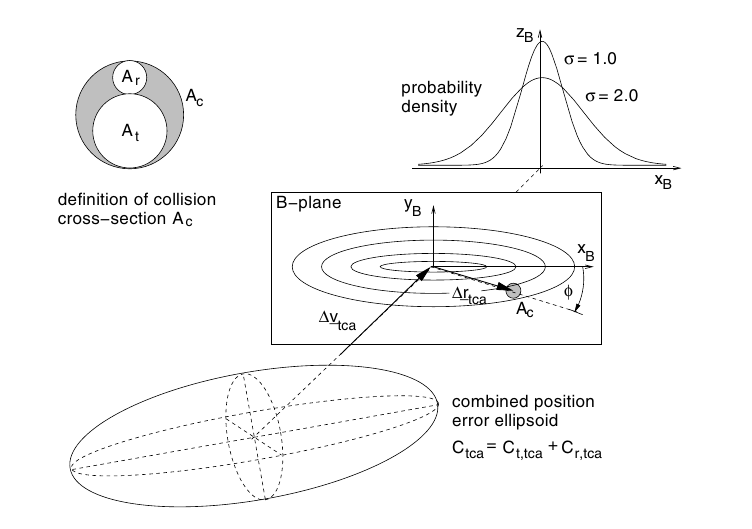
\includegraphics[width=0.5\textwidth]{imagenes/akellabplane}
 \caption{ B-plane (Adaptado de ....)}
 \label{fig:bplane}
\end{figure}

Bien, consideremos ahora una posici\'on relativa de acercamiento $\Delta r_{B}$ ya proyectada en el B-plane. La integral de volumen de la probabilidad de colisi\'on de la Eq. \ref{eq:poc3d} se reduce a una integral de superficie sobre la secci\'on circular de colisi\'on $R_{c}$, proyectada en el B-plane y centrada a la distancia relativa predicha en el instante de m\'aximo acercamiento, $\Delta r_{tca}$

\begin{equation}
P_{c} = \frac{1}{2 \pi \sqrt(det(C_{B}))} \int_{-R_{c}}^{+R_{c}} \int_{-\sqrt(R^{2}_{c}-x^{2}_{B})}^{+\sqrt(R^{2}_{c}-x^{2}_{B})} exp [- A_{B}] dy_{B} dx_{B}
\end{equation}

\begin{equation}
A_{B}=\frac{1}{2}\Delta r^{T}_{B} C^{-1}_{B} \Delta r_{B}
\end{equation}







